\quad \quad This subsystem will make various queries to the database as RFID tags become ready and 
display all the associated data to the Queue GUI. 

\begin{figure}[h!]
	\centering
 	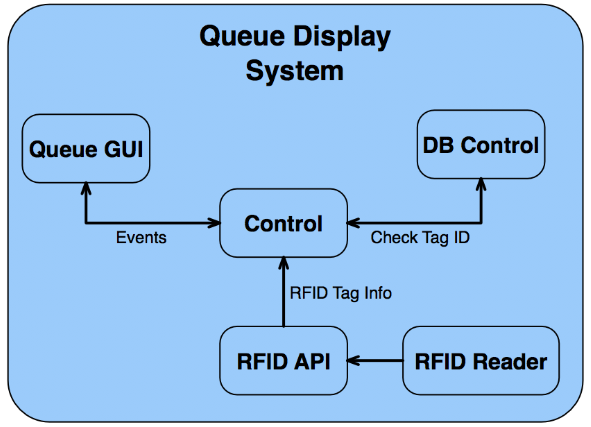
\includegraphics[width=0.60\textwidth]{images/ads_4}
 \caption{Queue Display Subsystems}
\end{figure}

\subsection{RFID API Subsystem}
\quad \quad The RFID API subsystem will communicate with the RFID Reader and take RFID tag ID to 
the control subsystem.

\subsubsection{Assumptions}
\quad \quad RFID tags have already been set up by the Student Management subsystem.

\subsubsection{Responsibilities}
\quad \quad This subsystem will identify the RFID tag that is scanned from the RFID Reader, 
utilizing the RFID API it will send the data to the Control model.

\subsubsection{Subsystem Interfaces}
\quad \quad This system has a single one-way interface, it parses the RFID tag from the reader 
into a format that the Control system can use.

\begin {table}[H]
\caption {Queue Display RFID API Subsystem interfaces} 
\begin{center}
    \begin{tabular}{ | p{1cm} | p{4cm} | p{4cm} | p{4cm} |}
    \hline
    ID & Description & Inputs & Outputs \\ \hline
    \#07 & RFID API & \pbox{4cm}{RFID Tag} & \pbox{4cm}{RFID Tag Info}  \\ \hline
    \end{tabular}
\end{center}
\end{table}

\subsection{Queue GUI Subsystem}
\quad \quad This subsystem handles all the data being displayed for the users to be able to 
successfully give the advanced notice for the staff to be able to dismiss the 
students.

\subsubsection{Assumptions}
\quad \quad The GUI has to be running at the same time and the database must have the data of 
the students who are assigned a RFID tag.

\subsubsection{Responsibilities}
\quad \quad This subsystem will handle events and triggers given by the control subsystem to be 
able to display all the relevant data of the student being picked up by the parent. 

\subsubsection{Subsystem Interfaces}
\quad \quad This subsystem will be a two way with regards to the control subsystem, it will send 
events to update the visualized data. 

\begin {table}[H]
\caption {Queue Display Queue GUI Subsystem interfaces} 
\begin{center}
    \begin{tabular}{ | p{1cm} | p{6cm} | p{3cm} | p{3cm} |}
    \hline
    ID & Description & Inputs & Outputs \\ \hline
    \#08 & Update Roster & \pbox{3cm}{User Input} & \pbox{3cm}{Events}  \\ \hline
    \#09 & Visualize Tag & \pbox{3cm}{GUI Data} & \pbox{3cm}{Screen Data}  \\ \hline
    \end{tabular}
\end{center}
\end{table}

\subsection{Control Subsystem}
\quad \quad This subsystem communicates with the database subsystem and the queue display 
subsystem and vice versa. It also reformats the data.

\subsubsection{Assumptions}
\quad \quad There has to be working input systems to get the user input and a database and GUI 
to handle the events.

\subsubsection{Responsibilities}
\quad \quad This subsystem handles the callback functions. It should act as a control unit 
between the GUI and the database. It also checks for the safe use for security.

\subsubsection{Subsystem Interfaces}
\quad \quad This system has three, two-way interfaces. The first is connected to the Queue GUI 
recieving GUI events and returning data to the GUI. The second 
passes and receives from DB Control. The Third takes data from the reader and pushes 
to the DB control, while the return is formatted to display in the GUI.

\begin {table}[H]
\caption {Queue Display Control Subsystem interfaces} 
\begin{center}
    \begin{tabular}{ | p{1cm} | p{5cm} | p{4cm} | p{3cm} |}
    \hline
    ID & Description & Inputs & Outputs \\ \hline
    \#10 & Control GUI & \pbox{4cm}{Events} & \pbox{3cm}{Database Query}  \\ \hline
    \#11 & Control Database & \pbox{4cm}{Database Response} & \pbox{3cm}{QUI Data}  \\ \hline
    \#12 & Readin Data & \pbox{4cm}{RDIF API Tag} & \pbox{3cm}{Database Query}  \\ \hline
	\end{tabular}
\end{center}
\end{table}

\subsection{DB Control Subsystem}
\quad \quad This subsystem handles all the data related to students needing to be dismissed by 
staff. This is the subsystem that handles forwarding and receiving information from 
the database.

\subsubsection{Assumptions}
\quad \quad All the data has been set up in the database and it should be receiving good data 
from the control sub system.

\subsubsection{Responsibilities}
\quad \quad This subsystem will return all the data requested by the Control subsystem querying 
the DB.

\subsubsection{Subsystem Interfaces}
\quad \quad This system has two, two-way interfaces. The first is connected to the database, 
sending queries and receiving responses.  The second passes and receives from Control.

\begin {table}[H]
\caption {Queue Display DB Control Subsystem interfaces} 
\begin{center}
    \begin{tabular}{ | p{1cm} | p{4cm} | p{4cm} | p{4cm} |}
    \hline
    ID & Description & Inputs & Outputs \\ \hline
    \#13 & Send Query & \pbox{4cm}{Database Query} & \pbox{4cm}{Query}  \\ \hline
    \#14 & Receive Results & \pbox{4cm}{Response} & \pbox{4cm}{Database Response}  \\ \hline
    \end{tabular}
\end{center}
\end{table}
